\documentclass[UTF8,a4paper,11pt]{ctexart}

\usepackage[margin=2.35cm]{geometry}
\usepackage{booktabs}
\usepackage{caption}
\usepackage{subcaption}
\usepackage{float}
\usepackage{graphicx}
\usepackage{hyperref}
\usepackage{enumitem}
\usepackage{xcolor}
\usepackage{array}

\graphicspath{{figures/}}
\hypersetup{
  colorlinks=true,
  linkcolor=blue!55!black,
  citecolor=blue!55!black,
  urlcolor=blue!55!black
}
\captionsetup{font=small,labelfont=bf}
\setlength{\parindent}{2em}
\setlength{\parskip}{0.25em}
\setlength{\emergencystretch}{2em}

\title{\textbf{监控人脸超分适用性报告}\\
\large GFPGAN、CodeFormer与Real-ESRGAN对比}
\author{吴止境}
\date{2026年7月}

\begin{document}

\pagestyle{plain}
\maketitle

\begin{abstract}
本报告在同一冻结协议下比较GFPGAN、CodeFormer（$w=1$）与Real-ESRGAN x2plus对远场监控人脸身份识别的影响。实验以MEVID actor check-in正面照建立固定ArcFace Gallery，对316条官方Query轨迹独立冻结face-best，并将所有后端输出统一归一化为112$\times$112后再提取ArcFace embedding。156条Query具有可对齐人脸，其中40条属于预先定义的recoverable组。该组原图Rank-1为26/40（65.0\%）；GFPGAN为8/40（20.0\%），CodeFormer为11/40（27.5\%），Real-ESRGAN为18/40（45.0\%）。两种纯缩放控制均保持26/40，排除了归一化过程本身导致下降的解释。GFPGAN与CodeFormer没有救回任何原图错误样本，分别使18条和15条原本正确样本退化；Real-ESRGAN救回1条、损害9条，仍比原图低20个百分点。三种算法均完成156/156次处理，但没有一种优于原图。结论是：当前产品身份识别默认应保留原始对齐脸；超分可用于人工画面增强和诊断实验，但不应未经独立校准直接替换ArcFace输入。

\textbf{关键词：}GFPGAN；CodeFormer；Real-ESRGAN；监控人脸；ArcFace；身份保持；超分
\end{abstract}

\section{结论}

三种超分算法都没有提高冻结recoverable组的ArcFace Rank-1。Real-ESRGAN x2plus在三者中最好，达到45.0\%，但仍比原图65.0\%低20个百分点；其PID聚类置换检验$p=0.312$，不能据此声称稳定改善。GFPGAN和CodeFormer分别降至20.0\%与27.5\%，且PID聚类置换检验均显示显著负向变化。两种只做放大再压回112$\times$112的控制组均保持65.0\%，说明下降来自超分模型改变了身份特征，而不是ArcFace输入归一化。

三种方法仍可改善人工查看体验或作为离线诊断工具。GFPGAN和CodeFormer使用生成式人脸先验，可能补出自然但不属于原身份的细节；Real-ESRGAN不使用专用人脸生成先验，身份漂移较小、速度也最快，但本次结果仍不支持把它设为默认身份前处理。

\begin{quote}
\textbf{身份识别默认使用原始对齐脸。GFPGAN、CodeFormer与Real-ESRGAN可以保留为可选画面增强，但在新的独立数据与身份保持校准给出正向证据前，不替换ArcFace输入。}
\end{quote}

\section{超分不适合作为默认识别前处理的风险}

\subsection{生成的合理细节不一定是真实细节}

GFPGAN不是普通插值。它先去除模糊、噪声和压缩痕迹，再利用预训练StyleGAN2中学到的人脸规律补充眼睛、皮肤、头发和轮廓\cite{gfpgan}。这种生成式人脸先验让它可以从很差的输入中得到自然结果。

GFPGAN在训练时加入了身份保持损失，希望修复前后仍然是同一个人\cite{gfpgan}。但是，当原图中的眼睛、皱纹或脸部边界已经无法辨认时，模型没有足够依据恢复真实细节，只能生成一个最合理的结果。

GFPGAN官方模型说明也列出了身份变化和美化倾向：V1.3可能产生轻微身份变化，V1.2的结果更锐利，但带有更明显的美化效果\footnote{\url{https://github.com/TencentARC/GFPGAN/blob/master/Comparisons.md}}。这说明视觉自然、清晰度和身份保持并不是同一个目标。

\subsection{像素太少时没有足够信息可恢复}

远场监控人脸经常只有十几或二十多个像素。此时眼睛、发际线、皱纹和脸部边界可能只剩几个像素。把图片放大到更高分辨率，只增加了输出像素，并没有增加摄像头当时记录到的信息。

同一张低清人脸可以对应多张不同的高清人脸。PULSE展示过，同一个低清输入可以生成多张看起来都合理、但人物外观不同的高清结果\cite{pulse}。这说明极低分辨率人脸不存在唯一恢复答案。

因此，超分必须有下限。没有检测到脸、疑似误检、极端姿态或小到无法确认五官的输入，不应进入GFPGAN，也不应继续判断身份。

\subsection{去噪和磨皮可能改写身份特征}

GFPGAN通常能较好地去除噪点和压缩痕迹，但也容易让皮肤变得平滑。额头细纹、眼周纹理、鼻唇沟和局部阴影可能被减弱或重新绘制。

噪点通常是干扰，去除噪点可能有利于识别。但稳定的轮廓、眼周结构和中尺度纹理可能与身份有关。GFPGAN无法始终准确区分“应该去掉的噪声”和“应该保留的真实纹理”。

图\ref{fig:einstein}中，修复图更干净、更锐利，但皱纹、皮肤颗粒和局部明暗也发生了变化。图像恢复研究已经证明，视觉质量提高可能伴随对原图忠实程度下降\cite{perceptiondistortion}。因此，图片看起来更清楚，不能直接说明ArcFace会识别得更准确。

\begin{figure}[H]
\centering
\begin{subfigure}[t]{0.36\textwidth}
  \centering
  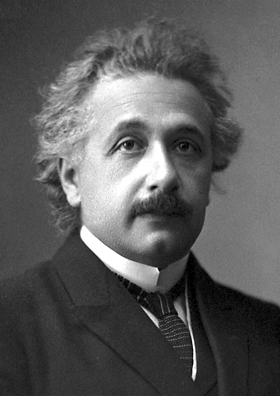
\includegraphics[height=6.8cm]{einstein_original_user.png}
  \caption{原图：皱纹、颗粒和局部明暗较明显}
\end{subfigure}
\hspace{0.06\textwidth}
\begin{subfigure}[t]{0.45\textwidth}
  \centering
  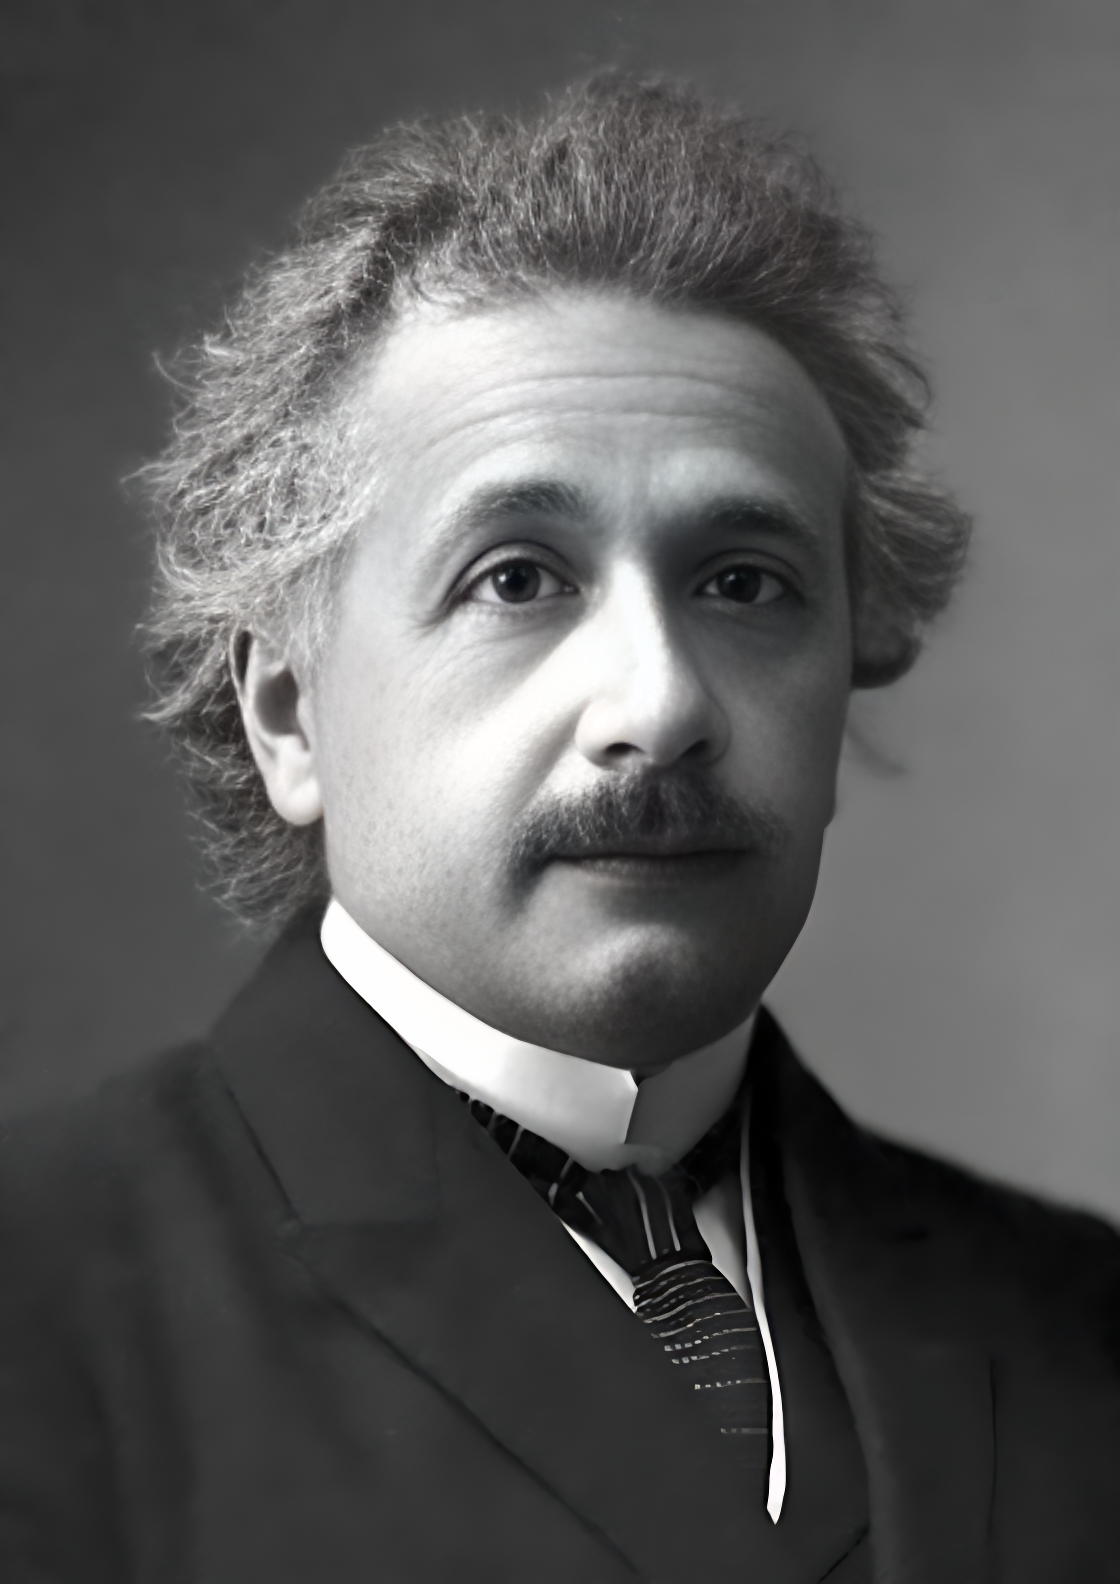
\includegraphics[height=6.8cm]{einstein_restored_user.png}
  \caption{修复图：噪声减少，但部分纹理被平滑或重绘}
\end{subfigure}
\caption{生成式修复同时带来去噪和纹理改写。该图用于说明现象，不作为定量实验结果。}
\label{fig:einstein}
\end{figure}

\section{CR-FIQA不能保证身份保持}

CR-FIQA用于预测一张人脸是否适合交给识别模型\cite{crfiqa}。我原本计划根据FIQA分数区分clear、marginal和poor，再决定是否建库、识别或超分。

我使用MEVID训练身份做过一次诊断。候选数据包含632条轨迹，其中118条得到有效人脸，最终形成39条参考记录和49条独立测试记录。

\begin{table}[H]
\centering
\caption{CR-FIQA在MEVID单帧协议中的诊断结果}
\label{tab:fiqa}
\begin{tabular}{lr}
\toprule
项目 & 结果\\
\midrule
ArcFace第一名正确 & 9/49（18.4\%）\\
第一名正确且达到0.45阈值 & 0/49\\
FIQA分数与是否认对的相关系数 & 0.026\\
不筛选时的第一名正确率 & 18.4\%\\
过滤最低10\% FIQA后 & 20.0\%\\
过滤最低20\% FIQA后 & 17.5\%\\
过滤最低50\% FIQA后 & 16.0\%\\
\bottomrule
\end{tabular}
\end{table}

FIQA高分人脸没有表现出更稳定的ArcFace识别结果。过滤最低10\%只产生轻微波动，继续过滤后识别率反而下降。因此，CR-FIQA不适合作为当前MEVID身份识别链路的单一决策依据。

多后端实验进一步验证了这一点。GFPGAN和CodeFormer使CR-FIQA平均分别增加0.468与0.154，但recoverable Rank-1分别下降45与37.5个百分点；Real-ESRGAN的FIQA平均下降0.142，Rank-1反而是三种超分中最高。CR-FIQA衡量单张人脸的潜在可识别性，但不能证明超分保留了同一身份。因此，本报告仅把FIQA作为诊断变量；在完成独立训练集与客户域校准前，FIQA不改变质量分桶、超分路由或C组成员，也不能把``FIQA上升''解释为``身份信息改善''。

\section{正式实验设计}

\subsection{固定Check-in Gallery与Query}

实验使用MEVID actor check-in正面照作为唯一人脸Gallery，不使用官方person ReID Gallery。Check-in压缩包含2,898张图片和172个数字前缀，覆盖全部104个train PID、54个test PID以及52个官方Query PID。官方资料没有单独发布映射表，因此实验同时保存编号覆盖审计与ArcFace sanity check，避免仅凭文件名假设映射。

Gallery只接收原始图中\texttt{direct + clear + can\_enroll=true}的人脸。最终选择343张check-in人脸，形成145个身份模板。52个Query PID中，0206和0294没有通过产品建库门控的check-in模板；结果保留这些Query并明确标记模板不可用，而不是静默删除。

316条官方Query轨迹均被纳入固定manifest。每条轨迹确定性均匀抽取24帧，用便宜的人体上部ROI代理维护Top-3候选，并加入body-best兜底；之后仅在候选上运行人脸检测和质量评估，使用产品共享的\texttt{face\_evidence\_rank}选择唯一face-best。选帧不读取身份预测结果。最终得到34条direct、40条recoverable、82条unusable和160条none。

\subsection{单轴质量分桶与双轴产品路由}

实验准备阶段考虑过两种设计。第一种设计只保留clear、marginal、poor和none质量类别，再把类别直接映射为原图识别、超分或拒绝。第二种设计同时输出质量类别和direct、recoverable、unusable、none可用状态。本实验采用第二种设计。这里的``双轴''不是运行两套互不相关的质量模型：两轴共享尺寸、检测置信度、姿态和模糊度等底层观测，但分别回答``图像质量如何''和``产品应采取什么动作''。

\begin{table}[H]
\centering
\caption{单轴质量类别驱动与双轴质量--可用状态设计对比}
\label{tab:quality-routing}
\renewcommand{\arraystretch}{1.18}
\begin{tabular}{p{0.17\textwidth}p{0.35\textwidth}p{0.38\textwidth}}
\toprule
设计 & 决策方式 & 优点与局限\\
\midrule
单轴类别驱动 &
先分为clear、marginal、poor和none，再为每个类别固定一种产品动作。 &
字段少、解释简单；但poor同时包含25像素可恢复小脸和8像素不可恢复小脸，marginal也可能同时包含可直接识别与值得尝试增强的样本。类别阈值变化会连带改变产品动作。\\
\addlinespace
双轴设计（采用） &
质量类别描述严重程度；可用状态根据缺陷类型和技术下限独立给出direct、recoverable、unusable或none。 &
能够区分``质量差但可处理''与``质量差且不可恢复''，便于安全拒绝、配置审计和冻结实验；代价是必须在文档和消费方中保持两类字段语义一致。\\
\bottomrule
\end{tabular}
\end{table}

具体而言，未检测到可用人脸时记为none；检测分数低于0.5、极端姿态，或人脸短边低于20像素时记为unusable。通过这些硬门槛后，短边位于20--28像素，或模糊程度落入配置化可恢复区间的人脸记为recoverable；其余可直接使用原图的人脸记为direct。质量类别不直接决定动作：一个poor样本可能因25像素小脸而recoverable，也可能因8像素小脸而unusable；一个marginal样本也可能保持direct。

冻结manifest生成时，156条可对齐Query均保存了CR-FIQA分数，但40条recoverable全部由20--28像素尺寸规则确定。反事实关闭FIQA后，这40条的成员完全不变；其中5条同时带有low-FIQA诊断标签，但该标签不是入组原因。因此，后续多超分后端实验继续复用相同manifest和eligibility，不重新分桶；超分前后FIQA只作为诊断统计，不参与C组路由或恢复后验收。

\subsection{固定多后端处理矩阵}

所有处理共享同一check-in Gallery、Query face-best、ArcFace和0.45接受阈值。CodeFormer fidelity固定为1.0，不在Query上调参\cite{codeformer}；Real-ESRGAN只运行通用x2超分，不调用GFPGAN或其他face enhancement\cite{realesrgan}。

\begin{table}[H]
\centering
\caption{固定A/B1--3/C1--3处理协议}
\label{tab:protocol}
\renewcommand{\arraystretch}{1.2}
\begin{tabular}{p{0.20\textwidth}p{0.70\textwidth}}
\toprule
组别 & 处理方式\\
\midrule
A：原图 & 所有已检测并对齐的face-best直接进入ArcFace；这是诊断对照，不代表产品会接受unusable样本。\\
B1/B2/B3 & 156张可对齐Query分别经过GFPGAN、CodeFormer $w=1$、Real-ESRGAN x2plus；失败时无向量，不回退A。\\
C1/C2/C3 & direct复用A，recoverable复用对应B，unusable和none无向量；只按冻结eligibility路由，FIQA不改变成员。\\
P-off & 描述性关闭组：direct和recoverable使用A，unusable和none无向量。\\
缩放控制 & 112$\rightarrow$512双线性或112$\rightarrow$224双三次插值，再以LANCZOS归一化为112$\times$112。\\
\bottomrule
\end{tabular}
\end{table}

GFPGAN与CodeFormer原生输出为512$\times$512，Real-ESRGAN原生输出为224$\times$224；三者均显式转换为RGB uint8并用Pillow LANCZOS归一化为112$\times$112后再进入ArcFace和FIQA。所有输入、配置、权重、缓存、图片与结果均保存SHA256。C组只从A/B缓存派生，不根据识别是否改善选择处理结果。

\section{正式实验结果}

\subsection{Recoverable主结果}

\begin{table}[H]
\centering
\caption{冻结recoverable 40条Query的身份识别结果}
\label{tab:multi-rank1}
\renewcommand{\arraystretch}{1.15}
\begin{tabular}{lrrrr}
\toprule
处理 & Rank-1 & Rank-5 & MRR & 相对A变化\\
\midrule
A原图 & \textbf{26/40（65.0\%）} & 28/40（70.0\%） & 0.693 & --\\
C1 GFPGAN & 8/40（20.0\%） & 12/40（30.0\%） & 0.259 & $-45.0$pp\\
C2 CodeFormer $w=1$ & 11/40（27.5\%） & 16/40（40.0\%） & 0.346 & $-37.5$pp\\
C3 Real-ESRGAN x2plus & 18/40（45.0\%） & 26/40（65.0\%） & 0.532 & $-20.0$pp\\
Resize512控制 & 26/40（65.0\%） & 29/40（72.5\%） & 0.690 & $0.0$pp\\
Resize-x2控制 & 26/40（65.0\%） & 29/40（72.5\%） & 0.688 & $0.0$pp\\
\bottomrule
\end{tabular}
\end{table}

原图在Rank-1上优于全部三种超分。Real-ESRGAN保留的身份信息最多，但仍低20个百分点；GFPGAN和CodeFormer下降更明显。两个缩放控制的Rank-1均与A完全相同，说明112$\rightarrow$高分辨率$\rightarrow$112的尺寸往返不是主要损失来源。

\begin{figure}[H]
\centering
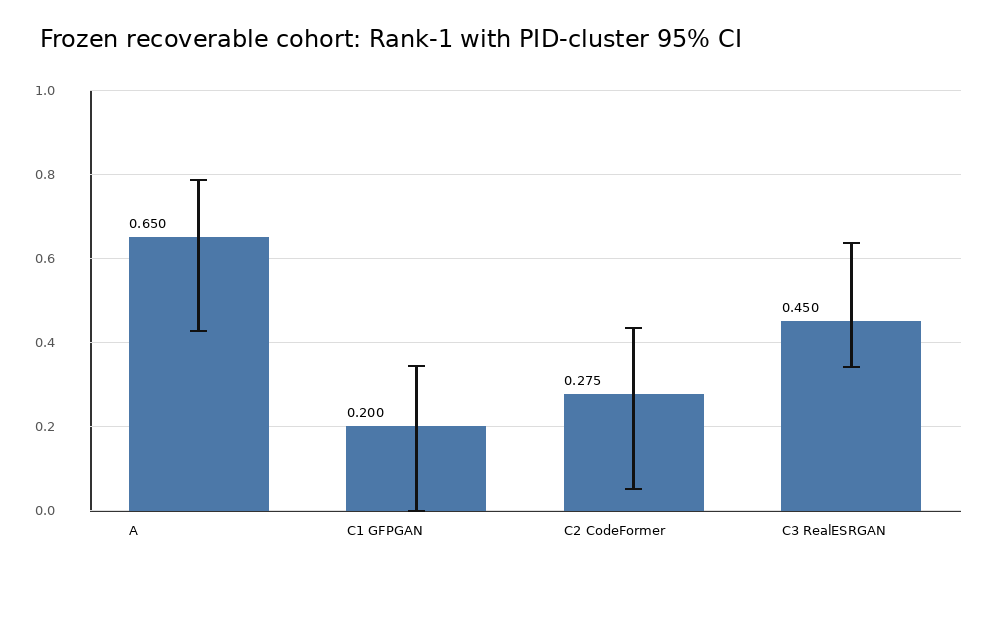
\includegraphics[width=0.88\textwidth]{recoverable_rank1_ci.png}
\caption{冻结recoverable组的Rank-1与PID聚类bootstrap 95\%置信区间。三种超分均低于原图；Real-ESRGAN最接近A，但置信区间仍显示较大不确定性。}
\label{fig:multi-rank1}
\end{figure}

\subsection{救回与损害的配对分析}

\begin{table}[H]
\centering
\caption{Recoverable组相对A的配对转换与PID聚类推断}
\label{tab:multi-paired}
\begin{tabular}{lrrrrr}
\toprule
方法 & 错$\rightarrow$对 & 对$\rightarrow$错 & 净变化 & 95\% CI & PID置换$p$\\
\midrule
GFPGAN & 0 & 18 & $-45.0$pp & $[-61.5,-33.3]$pp & 0.00125\\
CodeFormer & 0 & 15 & $-37.5$pp & $[-53.6,-25.0]$pp & 0.00410\\
Real-ESRGAN & 1 & 9 & $-20.0$pp & $[-33.3,+3.6]$pp & 0.31213\\
\bottomrule
\end{tabular}
\end{table}

GFPGAN和CodeFormer没有救回任何原图错误样本，却分别损害18条和15条原本正确样本；结论在PID聚类推断下仍为显著负向。Real-ESRGAN救回1条、损害9条，方向仍为负，但PID聚类置换$p=0.312$，不能把当前差异解释为稳定的人群级效应。这里的精确样本配对检验对Real-ESRGAN给出$p=0.0215$，但它没有处理同一PID多条Query之间的相关性，因此报告以PID聚类结果作为更保守依据。

\begin{figure}[H]
\centering
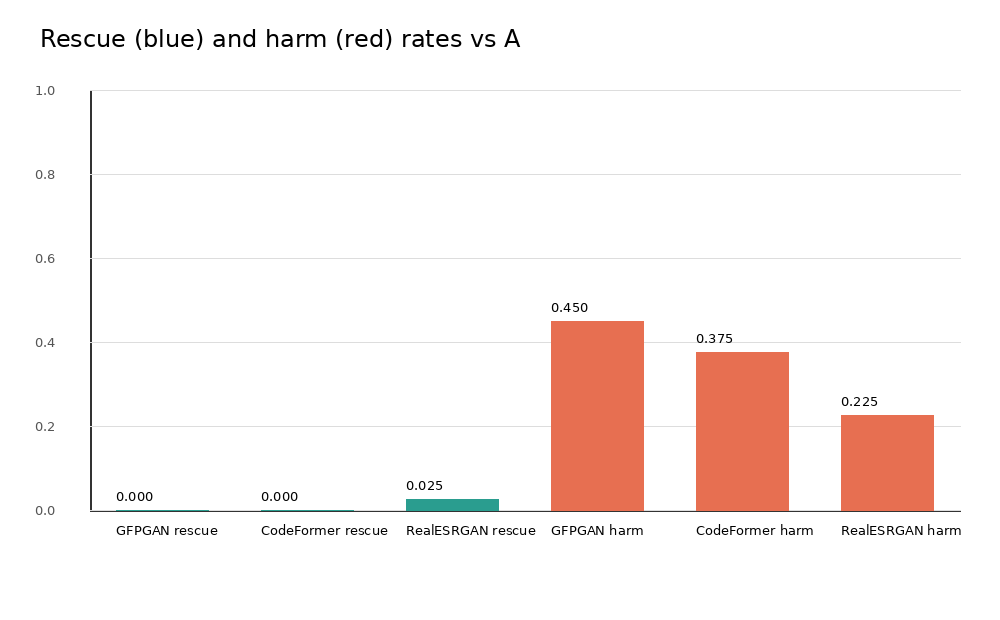
\includegraphics[width=0.92\textwidth]{rescue_harm_transitions.png}
\caption{相对A原图的救回率与损害率。GFPGAN和CodeFormer只有损害没有救回；Real-ESRGAN出现1条救回，但损害数量仍明显更多。}
\label{fig:rescue-harm}
\end{figure}

\subsection{全量后端运行、身份漂移与速度}

\begin{table}[H]
\centering
\caption{156张可对齐Query上的运行与诊断结果}
\label{tab:runtime}
\begin{tabular}{lrrrr}
\toprule
后端 & 成功/失败 & 平均秒/脸 & 原图--SR余弦 & FIQA平均变化\\
\midrule
GFPGAN & 156/0 & 0.236 & 0.402 & $+0.468$\\
CodeFormer $w=1$ & 156/0 & 0.324 & 0.584 & $+0.154$\\
Real-ESRGAN x2plus & 156/0 & \textbf{0.075} & \textbf{0.783} & $-0.142$\\
\bottomrule
\end{tabular}
\end{table}

表\ref{tab:runtime}的时间包含后端变换、normalize112、ArcFace embedding与FIQA诊断，不含一次性模型加载。Real-ESRGAN速度最快且与原图embedding最接近；GFPGAN身份漂移最大。FIQA变化方向与Rank-1排序并不一致：GFPGAN的FIQA提升最大，身份识别却最差；因此FIQA只保留为诊断，不用于C组路由。

\subsection{产品路由与三后端视觉对比}

在156张可对齐Query上，B1/B2/B3分别取得47、58和74条Rank-1正确；C1/C2/C3只保留34条direct原图和40条recoverable后端结果，因此分别取得37、40和47条Rank-1正确，并主动拒绝82条unusable。C的目标是执行冻结的安全路由，不是通过删除困难样本美化B的分数。

\begin{figure}[H]
\centering
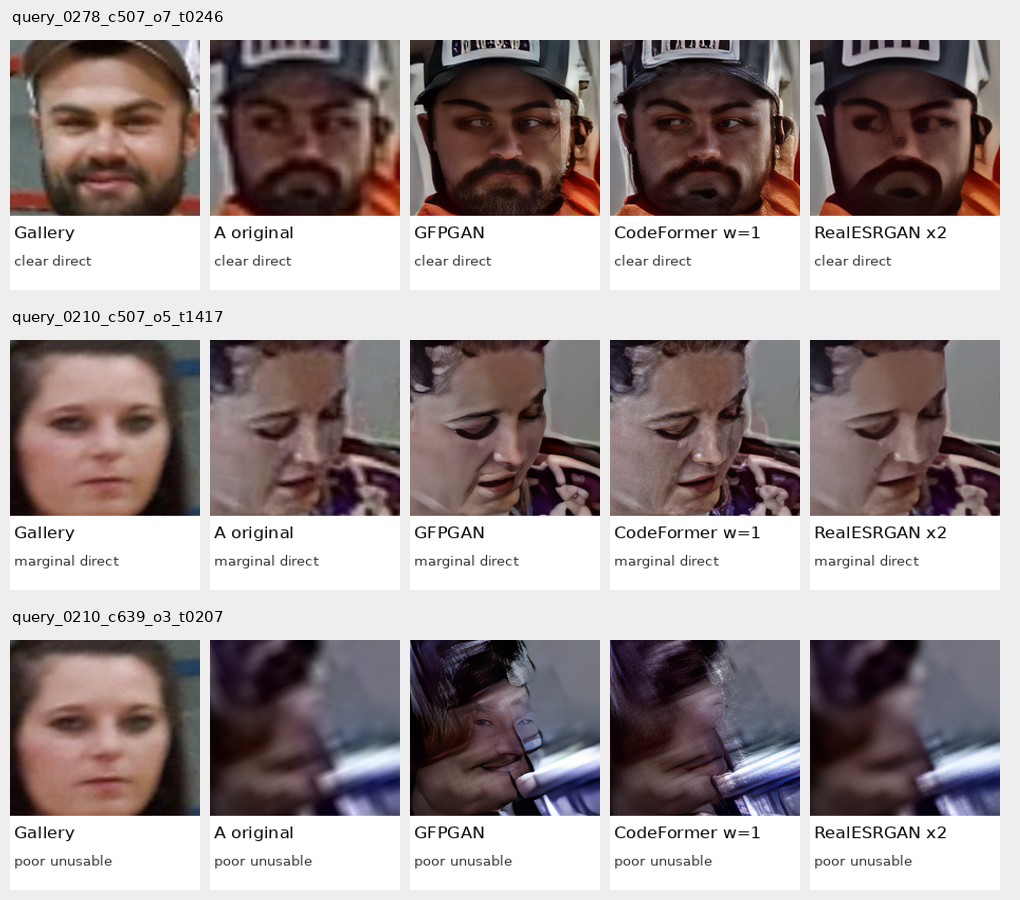
\includegraphics[width=\textwidth]{qualitative_grid.png}
\caption{三类冻结质量样本的统一视觉审计。每行按rule\_quality中位数确定，不读取识别结果；列为真实check-in Gallery、A原图、GFPGAN、CodeFormer $w=1$和Real-ESRGAN x2原生输出。视觉更清晰不等价于身份更稳定。}
\label{fig:qualitative-matrix}
\end{figure}

正式结果目录包含三后端及两种缩放控制各156张原生输出和156张normalize112图、40张recoverable逐样本面板、6张总览图、完整embedding与逐样本长表。2,126项结果checksum全部通过；三套权重SHA256分别为GFPGAN \texttt{c953a88f...a70}、CodeFormer \texttt{1009e537...84b7}、Real-ESRGAN \texttt{49fafd45...6abb}。本地归档SHA256为\texttt{06a0d71d...61b3}。

\section{限制}

\begin{enumerate}[leftmargin=2.2em]
  \item MEVID提供裁剪后的人体轨迹，本实验不能评价全帧人物检测、track ID switch或脸体关联精度；
  \item Check-in编号完整覆盖MEVID身份，且ArcFace sanity check支持对应关系，但官方没有单独发布actor-to-PID映射表；
  \item 52个Query PID中有两个没有合格的check-in模板；实验没有独立impostor Query，因此``错误接受''不能称为正式FMR；
  \item 结论针对GFPGAN V1.3、CodeFormer $w=1$、Real-ESRGAN x2plus、ArcFace和当前MEVID监控条件，不能推广为这些算法对所有画面修复任务都无效；
  \item recoverable主组只有40条Query。Real-ESRGAN的负向点估计尚未在PID聚类推断下达到显著，需要用更多独立身份和真实客户回放复验；
  \item CodeFormer使用S-Lab License 1.0，本实验仅作研究评估；任何商业产品使用前必须单独完成许可证审查。
\end{enumerate}

\section{产品建议}

现阶段，我建议：

\begin{enumerate}[leftmargin=2.2em]
  \item 身份识别默认关闭三种超分后端，direct与recoverable均优先使用原始对齐脸；unusable和none继续拒绝；
  \item 当前recoverable状态只表示输入达到技术处理下限，不表示任一超分算法能够恢复身份；
  \item 前端可保留GFPGAN、CodeFormer与Real-ESRGAN画面增强，并明确标记处理后图像；增强图不允许自动写入人脸Gallery；
  \item CR-FIQA保留为诊断信号；在独立校准证明其有效前，不用于改变质量分桶、超分路由或恢复后验收；
  \item 后续优先改进人脸感知选帧、多帧特征聚合和更高质量原始采集，再评估专门以身份保持为目标训练的超分方法。
\end{enumerate}

\footnotesize
\begin{thebibliography}{9}

\bibitem{gfpgan}
X. Wang, Y. Li, H. Zhang, and Y. Shan,
``Towards Real-World Blind Face Restoration with Generative Facial Prior,''
\textit{Proceedings of the IEEE/CVF Conference on Computer Vision and Pattern Recognition},
2021.

\bibitem{perceptiondistortion}
Y. Blau and T. Michaeli,
``The Perception-Distortion Tradeoff,''
\textit{Proceedings of the IEEE/CVF Conference on Computer Vision and Pattern Recognition},
2018.

\bibitem{pulse}
S. Menon, A. Damian, S. Hu, N. Ravi, and C. Rudin,
``PULSE: Self-Supervised Photo Upsampling via Latent Space Exploration of Generative Models,''
\textit{Proceedings of the IEEE/CVF Conference on Computer Vision and Pattern Recognition},
2020.

\bibitem{crfiqa}
F. Boutros, M. Fang, M. Klemt, B. Fu, and N. Damer,
``CR-FIQA: Face Image Quality Assessment by Learning Sample Relative Classifiability,''
\textit{Proceedings of the IEEE/CVF Conference on Computer Vision and Pattern Recognition},
2023.

\bibitem{codeformer}
S. Zhou, K. C. K. Chan, C. Li, and C. C. Loy,
``Towards Robust Blind Face Restoration with Codebook Lookup Transformer,''
\textit{Advances in Neural Information Processing Systems},
2022.

\bibitem{realesrgan}
X. Wang, L. Xie, C. Dong, and Y. Shan,
``Real-ESRGAN: Training Real-World Blind Super-Resolution with Pure Synthetic Data,''
\textit{Proceedings of the IEEE/CVF International Conference on Computer Vision Workshops},
2021.

\end{thebibliography}
\normalsize

\end{document}
